\chapter{Introduction}
\label{chap:introduction}

\section{Planetary defense}
\label{sec:planetary_defense}

The final law provided in Akin's Laws of Spacecraft Design states that \textit{"Space is a completely unforgiving environment. If you screw up the engineering, somebody dies."} \cite{akinslaws}. This law was written for engineers designing and building crewed space systems and it highlights the facts that space is an extremely hostile environment towards humans. However, the issue at hand is that space is also hostile to humans even when they are on their own planet. Of significant risk to planet Earth is a potential collision with a large asteroid or near-Earth object (NEO), which would cause extreme environmental phenomena such as massive tsunamis, multiple firestorms and potentially an impact winter caused by dust particles and debris rising to the stratosphere. All of this would ultimately lead to a mass extinction event, in which several species and life forms could not survive on the planet anymore. In fact, this has already happened once in the history of the Earth around 66 million years ago, when an object about 10 kilometers wide hit our planet in North America and triggered the \textit{Cretaceous-Paleogene} extinction event, which is the event that caused the extinction of most dinosaurs.

\subsection{Near-Earth Objects}
\label{ssec:neo}

Fortunately, unlike dinosaurs, humanity has created and developed resources dedicated to cataloging near-Earth objects, estimating the likelihood of Earth impacts and developing methods to avoid a potential collision. These resources are usually realized as a dedicated office within a larger government mandated space agency. Following the conventions used by the European Space Agency's Near-Earth Objects Coordination Centre (NEO), we can define \textbf{near-Earth objects} as asteroids or comets with a perihelion distance of \num{\leq1.3} \si{\astronomicalunit}, with comets having the additional requirement of having a period shorter than \num{200} years \cite{neo_definition}. Furthermore, we can define \textbf{Potentially Hazardous Asteroids (PHAs)} as asteroids that have a Earth Minimum Orbit Intersection Distance (MOID) of \num{0.05} \si{\astronomicalunit} or less, combined with an absolute magnitude $H$ of \num{22} or brighter \cite{neo_definition}. 


NASA's Jet Propulsion Laboratory has a dedicated Center for Near Earth Object Studies (CNEOS). CNEOS publishes rough statistics to monitor the progress of annual NEA discoveries, which can be seen in \Cref{fig:NEA_nasa}. By comparing JPL's data with data from IAU's Minor Planet Center, it can be determined that from \num{28500} objects discovered as of March 2022, \num{2271} of them are characterized as Potentially Hazardous Asteroids (PHAs) \cite{mpc_data}. 

\begin{figure}[h]
	\centering
	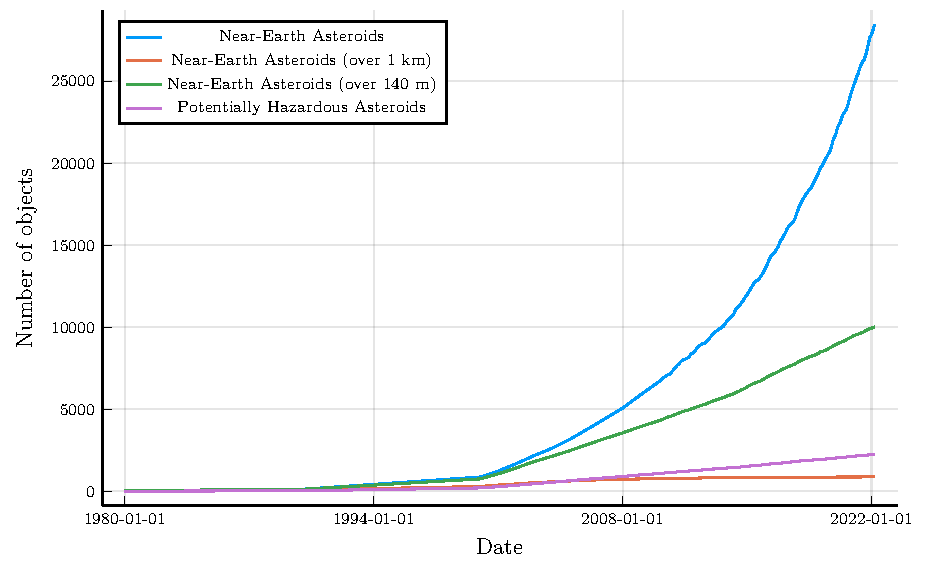
\includegraphics[width=\textwidth]{Figures/Chapter1/jpl_nea_data.pdf}
	\caption{Near-Earth Asteroids cataloged over the years. Today, about 8\% of them are classified as Potentially Hazardous Asteroids (data from \cite{nea_stats_jpl})}
	\label{fig:NEA_nasa}
\end{figure}


\begin{figure}[h]
	\centering
	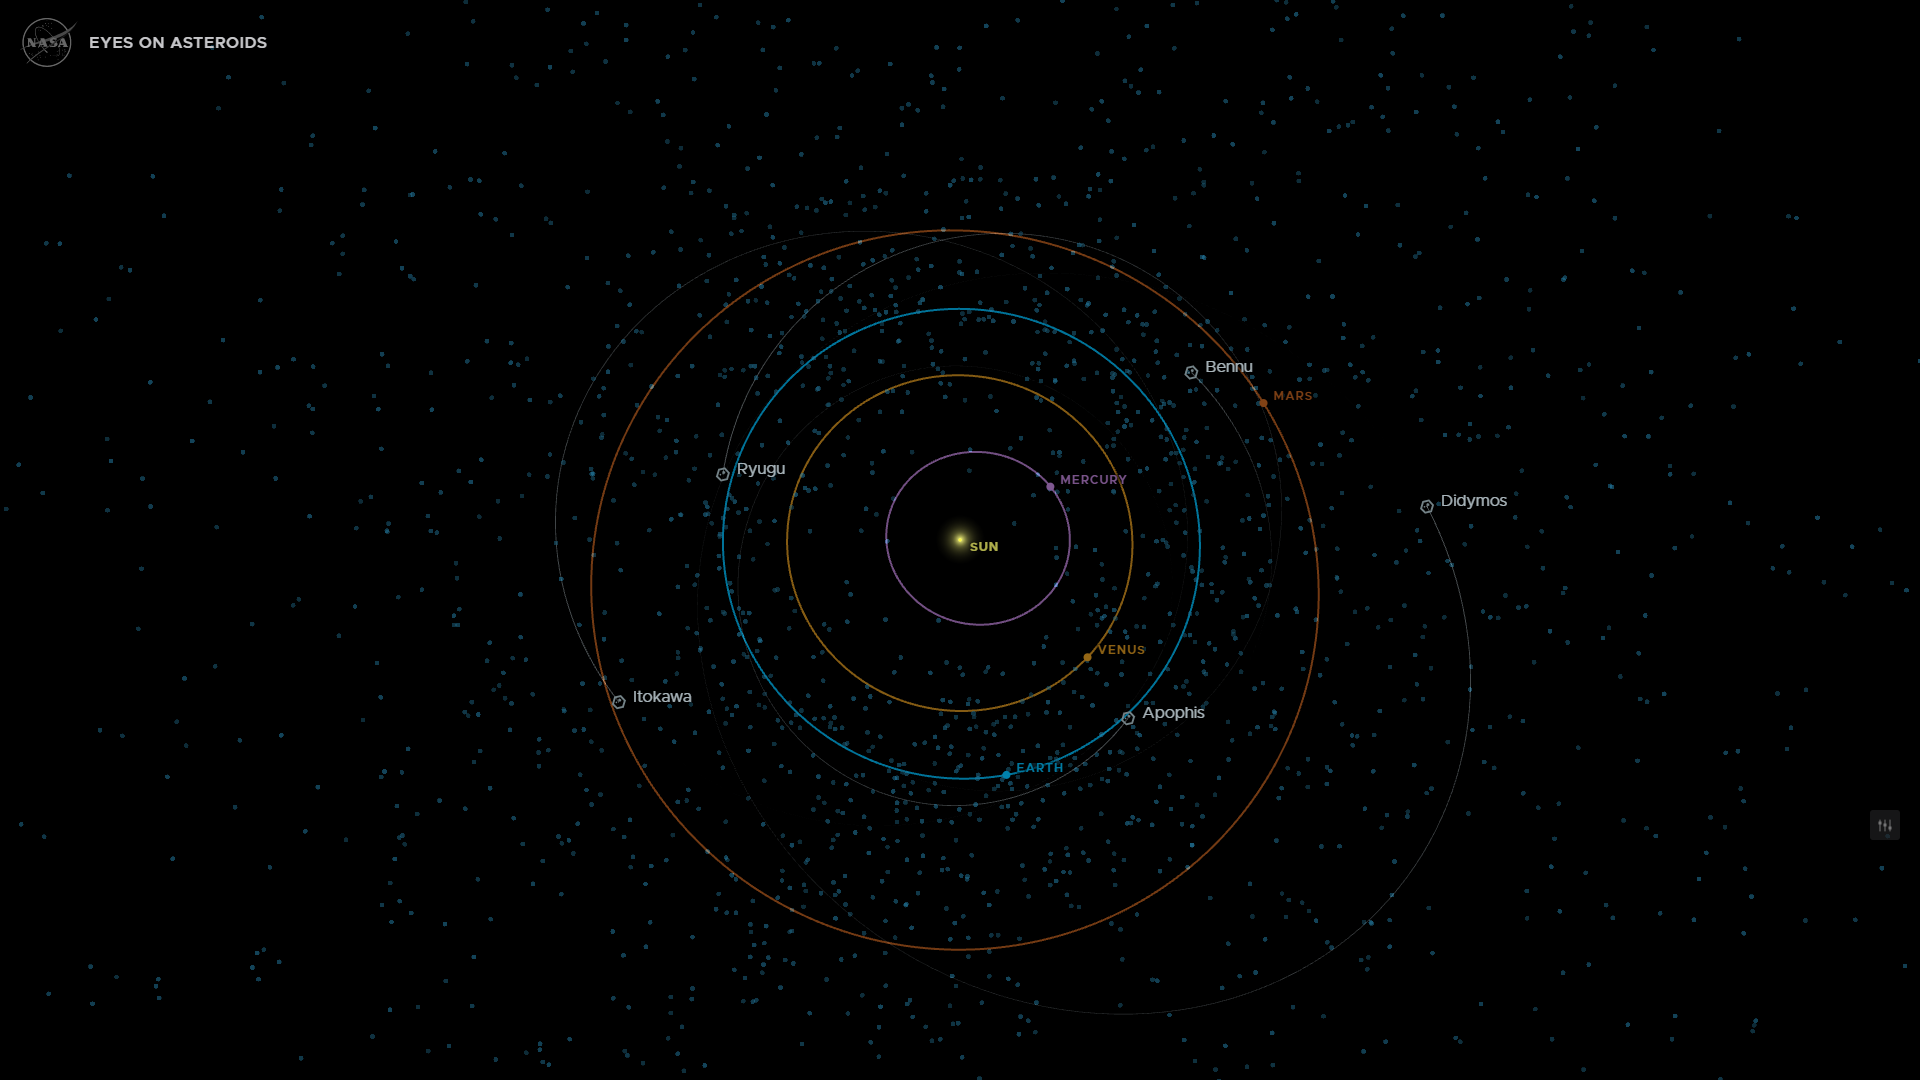
\includegraphics[width=\textwidth]{Figures/Chapter1/eyes_on_asteroids.png}
	\caption{Mapping of Potentially Hazardous Asteroids (as light blue points) for March 8th, 2022 (extracted from \cite{eyes_on_asteroids})}
	\label{fig:eyes_on_asteroids}
\end{figure}

\subsection{Techniques for collision avoidance}
\label{ssec:collision_avoidance}


\section{The Asteroid Impact and Deflection Assessment (AIDA)}